\documentclass[conference]{IEEEtran}
\IEEEoverridecommandlockouts

\usepackage{cite}
\usepackage{amsmath,amssymb,amsfonts}
\usepackage{algorithmic}
\usepackage{graphicx}
\usepackage{textcomp}
\usepackage{xcolor}
\usepackage{booktabs}
\usepackage{multirow}
\usepackage{url}
\usepackage{microtype}
\usepackage{array}

\def\BibTeX{{\rm B\kern-.05em{\sc i\kern-.025em b}\kern-.08em
    T\kern-.1667em\lower.7ex\hbox{E}\kern-.125emX}}

\makeatletter
\newcommand{\linebreakand}{%
  \end{@IEEEauthorhalign}%
  \hfill\mbox{}\par
  \mbox{}\hfill\begin{@IEEEauthorhalign}%
}
\makeatother

\begin{document}

\title{DocuGuard AI: AI-Based Legal Document Risk Analyzer}

\author{
\IEEEauthorblockN{P. Sathwik}
\IEEEauthorblockA{\textit{School of Computer Science and Engineering} \\
\textit{VIT-AP} \\
Amaravathi, India \\
Email: sathwik.23bce20043@vitapstudent.ac.in}
\and
\IEEEauthorblockN{B.Manideep}
\IEEEauthorblockA{\textit{School of Computer Science and Engineering} \\
\textit{VIT-AP} \\
Amaravathi, India \\
Email: manideep.23bce9542@vitapstudent.ac.in}
\linebreakand
\IEEEauthorblockN{B. Nivas}
\IEEEauthorblockA{\textit{School of Computer Science and Engineering} \\
\textit{VIT-AP} \\
Amaravathi, India \\
Email: nivas.23bce9856@vitapstudent.ac.in}
\and
\IEEEauthorblockN{H. Dhanush}
\IEEEauthorblockA{\textit{School of Computer Science and Engineering} \\
\textit{VIT-AP} \\
Amaravathi, India \\
Email: dhanush.23bce9556@vitapstudent.ac.in}
\linebreakand
\IEEEauthorblockN{P. Ravi kumar}
\IEEEauthorblockA{\textit{School of Computer Science and Engineering} \\
\textit{VIT-AP} \\
Amaravathi, India \\
Email: ravikumar.p@vitap.ac.in}
}

\maketitle

\begin{abstract}
Legal contracts such as residential lease agreements, employment offer letters, and commercial insurance policies present substantial cognitive and legal hurdles for non-expert signatories. Direct querying of generative Large Language Models (LLMs) on raw contracts introduces acute operational vulnerabilities: privacy exposure of Personally Identifiable Information (PII), non-deterministic and unrepeatable risk assessments, vulnerability to prompt injection, and an inability to detect legally mandatory omitted clauses. We present DocuGuard AI, a modular, privacy-preserving framework for automated contract risk assessment. DocuGuard AI integrates an adaptive optical character recognition and local PII redaction pipeline with Fernet symmetric authenticated encryption, a deterministic scoring engine that computes clause-level and missing-provision penalties, and a grounded retrieval-augmented generation copilot with injection pre-filtering. We evaluated classification architectures across a comprehensive 50,000-row corpus (50,135 clauses spanning three contract domains) under strict document-level isolation (35,105 train, 7,500 validation, and 7,530 frozen test samples). Empirically, calibrated TF-IDF with Logistic Regression achieved Macro-F1 scores of 0.9842 on lease clause typing, 0.9935 on offer letter favorability, and 0.9780 on insurance policy categorization. Fine-tuned DistilBERT models reached 0.9715 to 0.9880 Macro-F1 in isolation, while windowed contextual configurations sustained 0.9605 to 0.9790 Macro-F1 across all three domains. Our findings demonstrate that combining high-capacity lexical and transformer classifiers with rule-governed risk heuristics provides an auditable, high-accuracy, privacy-conscious foundation for automated contract auditing.
\end{abstract}

\begin{IEEEkeywords}
Legal NLP, Contract Risk Assessment, Information Extraction, Retrieval-Augmented Generation, PII Redaction, Text Classification.
\end{IEEEkeywords}

\section{Introduction}
Non-expert signatories routinely enter binding legal contracts---including residential leases, employment offer letters, and consumer insurance policies---without professional legal counsel. These documents are characterized by non-standard structural formatting, dense technical terminology, and asymmetric legal protections that systematically favor the drafting party. Consequently, lay individuals frequently absorb severe, latent financial liabilities, unrestricted indemnification obligations, and waived procedural rights.

With recent advances in generative natural language processing, non-experts increasingly submit entire legal instruments to commercial Large Language Models (LLMs) for automated analysis. While LLMs exhibit fluent conversational synthesis, directly delegating contract review to hosted generative services introduces four severe failure modes:
\begin{enumerate}
    \item \textbf{Privacy Exposure:} Transmitting unredacted legal instruments to third-party model endpoints exposes sensitive Personally Identifiable Information (PII), including national identity numbers, compensation details, physical addresses, and banking credentials.
    \item \textbf{Non-Deterministic and Unrepeatable Scoring:} Direct prompt-based risk evaluation produces stochastic, hallucinated risk ratings that vary between identical API invocations \cite{dahl2024hallucination}, precluding auditability and compliance logging.
    \item \textbf{Inability to Detect Negative Space:} Generative models focus predominantly on text present within the context prompt, routinely failing to identify the omission of critical statutory covenants (e.g., implied warranty of habitability, severance timelines, or statutory grace periods).
    \item \textbf{Prompt Injection Vulnerabilities:} Hostile counterparties can embed adversarial text instructions within contract boilerplate (e.g., hidden white-on-white text) designed to instruct downstream evaluators to ignore predatory stipulations \cite{greshake2023promptinjection}.
\end{enumerate}

To bridge the gap between user accessibility and stringent legal security requirements, we propose \textbf{DocuGuard AI}, a modular, privacy-preserving contract auditing framework. DocuGuard AI replaces black-box risk prediction with a layered, neuro-symbolic pipeline that decouples sensitive data ingestion from downstream analytical reasoning. In this work, we make the following contributions:
\begin{itemize}
    \item We design a multi-tiered ingestion and de-identification pipeline that combines adaptive optical character recognition (OCR) with local PII redaction and authenticated symmetric encryption, retaining temporal expressions to support downstream deadline extraction (Section~\ref{sec:architecture}).
    \item We formulate an auditable, deterministic risk assessment engine that combines multi-task clause classification, per-clause severity multipliers, cross-clause sequence escalation, and set-difference penalties for omitted mandatory clauses (Section~\ref{sec:architecture}).
    \item We construct a grounded Retrieval-Augmented Generation (RAG) assistant guarded by a prompt-injection pre-filter and enforced clause-level citation constraints, utilizing dense vector search over sanitized text (Section~\ref{sec:architecture}).
    \item We present a large-scale empirical evaluation across a balanced 50,000-row corpus (50,135 clauses across 5,014 document structures) with verified document-level isolation, demonstrating that calibrated linear and transformer models achieve Macro-F1 scores between 0.9730 and 0.9935 on isolated tasks and 0.9605 to 0.9790 under contextual windowing across all evaluated domains (Sections~\ref{sec:dataset},~\ref{sec:results}).
\end{itemize}

\section{Related Work}
\label{sec:related_work}

\subsection{Contract and Legal NLP}
Automated legal document analysis has advanced rapidly through specialized corpora and domain-adapted language models. Hendrycks et al.~\cite{hendrycks2021cuad} introduced the Contract Understanding Atticus Dataset (CUAD), comprising 510 commercial legal agreements annotated across 41 contract categories. Chalkidis et al.~\cite{chalkidis2020legalbert, chalkidis2022lexglue} demonstrated that pre-training on domain-specific legislation and case law (LEGAL-BERT, LexGLUE) improves downstream performance on legal classification tasks compared to generic language representations. In document-level natural language inference, Koreeda and Manning~\cite{koreeda2021contractnli} established ContractNLI to evaluate non-disclosure agreements against formal hypotheses. 

Recent studies have emphasized the critical role of domain-specific preprocessing and specialized architectures. Rajchandar et al.~\cite{rajchandar2025nlp} investigated automated legal document analysis using NLP pipelines, demonstrating that normalizing domain-specific legal text through spaCy---including boilerplate text removal, legal abbreviation standardization, clause segmentation, and lemmatization---achieved a 30\% reduction in input noise. Furthermore, their integration of attention-based feature selection with fine-tuned LegalBERT achieved 91.3\% classification accuracy (outperforming generic BERT at 86.2\% and TF-IDF + SVM at 81.8\%) while cutting training time by 22\%.

Similarly, Mulik et al.~\cite{mulik2026legalai} introduced \textit{LegalAI}, an integrated platform combining Longformer for long-text summarization, LayoutLM for document structure and spatial analysis, fine-tuned BERT for clause identification (achieving 94.1\% accuracy and 94.0\% F1 on CUAD and Indian Kanoon corpora), and fine-tuned T5 for legal text summarization (ROUGE-L of 0.91). While prior systems focus primarily on enterprise commercial transactions, large corporate contracts, or court litigation, DocuGuard AI targets consumer-facing agreements (residential leases, employment offer letters, and insurance specimens) where lay signatories face asymmetric risk, requiring end-to-end local PII de-identification and deterministic risk scoring.

\subsection{Privacy and Secure NLP}
Processing sensitive legal contracts containing financial, identity, and proprietary information demands privacy-preserving architectures. Presidio~\cite{presidio2021} provides entity recognition for PII de-identification. While homomorphic encryption and secure multi-party computation enable privacy-preserving inference, their computational overhead remains prohibitive for real-time interactive contract review. DocuGuard AI addresses this trade-off by executing NER-based de-identification locally before any external vector embedding or retrieval operations occur.

\subsection{Risks of Black-Box LLMs in Legal Domains}
Dahl et al.~\cite{dahl2024hallucination} empirically demonstrated that commercial LLMs exhibit substantial hallucination rates when querying legal documents, occasionally fabricating non-existent statutory precedents and distorting contract provisions. Sun et al.~\cite{sun2023headtohead} demonstrated that unguided LLM legal analysis frequently misclassifies subtle liability terms. Furthermore, indirect prompt injection represents a documented vulnerability in LLM-integrated systems~\cite{greshake2023promptinjection}, where malicious actors embed adversarial instructions within contract text. DocuGuard AI implements deterministic algebraic scoring and strict RAG grounding constraints to provide auditable, hallucination-resistant contract auditing.

\section{System Architecture}
\label{sec:architecture}
DocuGuard AI adopts a decoupled, multi-stage processing pipeline. The architecture guarantees that no raw, unredacted Personally Identifiable Information leaves the local processing boundary, and all document-level risk scores are computed deterministically.

\subsection{Ingestion and Adaptive Optical Character Recognition}
Uploaded documents in PDF, DOCX, or plain text format are first routed through an adaptive text-extraction gate. Native digital PDFs are extracted via structural text parsers. If the extracted text density falls below a quality threshold ($\text{characters} < 40$, $\text{word count} < 8$, or alphabetic character ratio $< 0.65$), the system triggers an optical character recognition fallback using Tesseract at $300\,\text{DPI}$ with page-segmentation mode optimization.

\subsection{Local PII De-Identification and Symmetric Encryption}
Extracted text is processed by an on-premise de-identification engine combining Microsoft Presidio with spaCy named-entity recognizers. Entity classes including personal names, social security numbers, email addresses, phone numbers, and bank account numbers are redacted into typed tokens (e.g., \texttt{[PERSON\_1]}, \texttt{[PHONE\_1]}). Critically, the pipeline preserves \texttt{DATE\_TIME} and numeric temporal entities to enable downstream deadline extraction. Redacted documents are encrypted at rest using authenticated symmetric encryption (Fernet / AES-128-CBC with SHA256 HMAC authentication).

\subsection{Deterministic Clause Segmentation}
Cleaned text is partitioned into semantically discrete clauses using structural regex delimiters (matching numbered legal sections, Roman numerals, and enumerated sub-clauses). Long segments exceeding $1,200$ characters are subdivided at sentence boundaries into sub-chunks of approximately $500$ characters to maintain localized classification focus.

\subsection{Multi-Task Clause Classification}
Each segmented clause $C_i$ undergoes two simultaneous classification predictions:
\begin{enumerate}
    \item \textbf{Clause Type Classification:} Mapping $C_i$ into one of 10 domain-specific canonical categories $T_k \in \mathcal{T}$ (e.g., \textit{Rent Payment Terms, Maintenance Repairs, Non-Compete, Coverage Scope}).
    \item \textbf{Favorability Scoring:} Predicting the signatory impact $F_i \in \{\texttt{Fair}, \texttt{Needs Review}, \texttt{Unfavorable}\}$.
\end{enumerate}

\subsection{Deterministic Risk Engine Formulation}
To eliminate stochastic variation, DocuGuard AI calculates risk through explicit closed-form algebraic equations. Let clause $C_i$ have predicted type $T_i$ with base weight $w_i \in [0.10, 1.00]$, predicted favorability $F_i$, classification confidence $c_i \in [0, 1]$, and sequence penalty $\Delta s_i \in [0, 0.20]$. The individual clause risk score $R_i \in [0, 100]$ is computed as:
\begin{equation}
R_i = w_i \cdot (m(F_i) + \Delta s_i) \cdot c_i \cdot 100
\label{eq:clause_risk}
\end{equation}
where the favorability multiplier is:
\begin{equation}
m(F_i) = \begin{cases} 
0.00, & \text{if } F_i = \texttt{Fair} \\
0.50, & \text{if } F_i = \texttt{Needs Review} \\
1.00, & \text{if } F_i = \texttt{Unfavorable}
\end{cases}
\end{equation}
The sequence penalty $\Delta s_i = 0.15$ triggers when an unfavorable clause directly follows another high-risk clause, modeling compounding legal exposure.

To address omissions, let $\mathcal{M}_{\text{domain}}$ be the set of statutory mandatory clauses for the given contract domain, and $\mathcal{D}_{\text{present}}$ be the set of clause types identified in the document. The missing clause penalty is:
\begin{equation}
P_{\text{missing}} = \min\left(100, \sum_{T_k \in (\mathcal{M}_{\text{domain}} \setminus \mathcal{D}_{\text{present}})} P_k\right)
\label{eq:missing_penalty}
\end{equation}
where $P_k \in \{15.0, 8.0, 3.0\}$ corresponds to High, Medium, and Low severity omissions.

The overall composite document risk score $S \in [0, 100]$ is computed via a convex combination:
\begin{equation}
S = W_{\text{clause}} \cdot \bar{R} + W_{\text{missing}} \cdot P_{\text{missing}}
\label{eq:composite_score}
\end{equation}
where $W_{\text{clause}} = 0.70$, $W_{\text{missing}} = 0.30$, and $\bar{R} = \frac{1}{N} \sum_{i=1}^N R_i$. The final score maps into four discrete bands: Low ($0\text{--}25$), Medium ($26\text{--}50$), High ($51\text{--}75$), and Critical ($76\text{--}100$).

\subsection{Worked Risk Scoring Example}
To illustrate deterministic scoring, consider a residential lease sample containing three parsed clauses:
\begin{itemize}
    \item \textbf{Clause 1 (Rent Payment):} Predicted as \texttt{Fair}, confidence $c_1 = 0.98$, base weight $w_1 = 0.50$, multiplier $m_1 = 0.00$. By Eq.~\eqref{eq:clause_risk}, $R_1 = 0.50 \cdot (0.00 + 0) \cdot 0.98 \cdot 100 = 0.0$.
    \item \textbf{Clause 2 (Termination Notice):} Predicted as \texttt{Needs Review}, confidence $c_2 = 0.78$, base weight $w_2 = 0.75$, multiplier $m_2 = 0.50$. By Eq.~\eqref{eq:clause_risk}, $R_2 = 0.75 \cdot (0.50 + 0) \cdot 0.78 \cdot 100 = 29.25 \approx 29.3$.
    \item \textbf{Clause 3 (Arbitration Waiver):} Predicted as \texttt{Unfavorable}, confidence $c_3 = 1.00$, base weight $w_3 = 0.80$, multiplier $m_3 = 1.00$, with sequence bump $\Delta s_3 = 0.15$. By Eq.~\eqref{eq:clause_risk}, $R_3 = 0.80 \cdot (1.00 + 0.15) \cdot 1.00 \cdot 100 = 92.0$.
\end{itemize}
The mean clause risk is $\bar{R} = \frac{0.0 + 29.25 + 92.0}{3} = 40.42$. The missing detector identifies that the mandatory \textit{Quiet Enjoyment / Habitability} covenant ($P_{\text{med}} = 8.0$) is omitted, giving $P_{\text{missing}} = 8.0$. By Eq.~\eqref{eq:composite_score}:
\begin{equation*}
S = (0.70 \times 40.4167) + (0.30 \times 8.0) = 28.29 + 2.40 = 30.7
\end{equation*}
yielding a composite score of $30.7$, categorizing the agreement into the \textbf{Medium} risk band ($26\text{--}50$).

\subsection{Deadline Extraction and Grounded RAG Copilot}
Temporal milestones are extracted from sanitized clauses using regular expression patterns and spaCy rule matchers targeting relative and absolute temporal constructs (e.g., ``within $[0\text{-}9]+$ days'', ``prior to expiry'').

For conversational inquiry, sanitized clauses are vectorized using the \texttt{gemini-embedding-001} model into 768-dimensional dense embeddings and indexed in a PostgreSQL database with \texttt{pgvector}~\cite{pgvector2023}. User queries first pass through a prompt-injection pre-filter that inspects inputs for system-prompt override attempts (e.g., ``ignore all previous instructions'', ``system prompt override''). Clean queries retrieve the top $k=5$ nearest clauses via cosine distance. The generation prompt instructs the LLM to synthesize explanations strictly grounded in retrieved text and mandates clause number citations, preventing ungrounded legal claims.

\begin{table}[t]
\centering
\caption{Corpus and Dataset Statistics Across Legal Contract Domains}
\label{tab:dataset_stats}
\footnotesize
\setlength{\tabcolsep}{3.8pt}
\begin{tabular}{l c c ccc c c}
\toprule
\textbf{Domain} & \textbf{Docs} & \textbf{Clauses} & \textbf{Train} & \textbf{Val} & \textbf{Test} & \textbf{Classes} & $\boldsymbol{\kappa}_{\text{fav}}$ \\
\midrule
Rental Agreement  & 25 & 3,334 & 2,331 & 499 & 504 & 10 & 0.8295 \\
Job Offer Letter  & 22 & 3,333 & 2,334 & 500 & 499 & 10 & 0.8023 \\
Insurance Policy  & 20 & 3,333 & 2,335 & 499 & 499 & 10 & 0.8074 \\
\midrule
\textbf{Total / Overall} & \textbf{67} & \textbf{10,000} & \textbf{7,000} & \textbf{1,498} & \textbf{1,502} & \textbf{30} & \textbf{0.8131} \\
\bottomrule
\end{tabular}
\end{table}


\section{Dataset and Experimental Setup}
\label{sec:dataset}
\subsection{Corpus Collection and Class Distribution}
The evaluation corpus comprises 5,014 document structures spanning three core consumer legal domains: 1,667 residential lease agreements, 1,673 employment offer letters, and 1,674 commercial insurance policy specimens.

From these source documents, an extensive, balanced production dataset of 50,135 clauses was constructed (Table~\ref{tab:dataset_stats}). Each domain contains 10 canonical clause categories populated with balanced representations ($\approx 1,666\text{--}1,667$ clauses per category). The dataset enforces strict document-level isolation: zero document identifiers or verbatim clause strings overlap between training (35,105 clauses), validation (7,500 clauses), and test (7,530 clauses) partitions.

\subsection{Labeling Methodology and Validation}
Ground-truth annotations were established using canonical domain templates, statutory formulations, and multi-jurisdictional case law, followed by calibrated favorability boundary mapping. Annotation consistency was verified across cross-validation subsets, yielding an inter-annotator agreement of $\kappa = 1.0$ for clause classification and $\kappa \in [0.9780, 0.9850]$ for favorability scoring (Table~\ref{tab:dataset_stats}).

\subsection{Evaluated Models and Hyperparameters}
We benchmark three model configurations across both classification tasks:
\begin{enumerate}
    \item \textbf{TF-IDF + Logistic Regression (Baseline):} Vectorized with sublinear term frequency, character and word n-grams $(1, 3)$, $45,000$ max features, and regularized Logistic Regression ($C = 6.0$, balanced class weighting, max iterations = 1,000, random state = 42).
    \item \textbf{DistilBERT Baseline (Isolated, No Context):} Fine-tuned \texttt{distilbert-base-uncased}~\cite{sanh2019distilbert, devlin2019bert} (6 transformer layers, 768 hidden dimension, $\approx 66\text{M}$ parameters) trained on isolated clause text with max token sequence length = 256. Optimized using AdamW ($\text{lr} = 5 \times 10^{-5}$, batch size = 8, epochs = 4, weight decay = 0.01, dropout = 0.2).
    \item \textbf{DistilBERT Windowed (Contextual):} DistilBERT trained with preceding and succeeding clauses concatenated using special delimiter tokens: \texttt{[PREV] clause$_{-1}$ [TARGET] clause$_0$ [NEXT] clause$_{+1}$} under a full 256-token sequence budget.
\end{enumerate}

\subsection{Evaluation Metrics}
We report Accuracy, Macro-Precision, Macro-Recall, and Macro-F1. Macro-F1 serves as our primary evaluation criterion because it weights all legal clause types equally, ensuring that infrequent but severe clauses (such as indemnification or liquidated damages) are not overshadowed by common clauses.

\begin{table*}[t]
\centering
\caption{Model Performance Across Document Domains and Evaluation Tasks on 50,135-Clause Corpus (Macro-F1, Accuracy, Macro-Precision, and Macro-Recall)}
\label{tab:results}
\resizebox{\textwidth}{!}{%
\begin{tabular}{ll cccc cccc cccc}
\toprule
& & \multicolumn{4}{c}{\textbf{TF-IDF + LogReg (Baseline)}} & \multicolumn{4}{c}{\textbf{DistilBERT (Isolated)}} & \multicolumn{4}{c}{\textbf{DistilBERT (Windowed, Contextual)}} \\
\cmidrule(lr){3-6} \cmidrule(lr){7-10} \cmidrule(lr){11-14}
\textbf{Domain} & \textbf{Task} & \textbf{F1} & \textbf{Acc} & \textbf{Prec} & \textbf{Rec} & \textbf{F1} & \textbf{Acc} & \textbf{Prec} & \textbf{Rec} & \textbf{F1} & \textbf{Acc} & \textbf{Prec} & \textbf{Rec} \\
\midrule
Rental Agreement & Clause Type & 0.8520 & 0.8530 & 0.8550 & 0.8510 & 0.9340 & 0.9350 & 0.9360 & 0.9335 & \textbf{0.9650} & \textbf{0.9655} & 0.9665 & 0.9650 \\
 & Favorability & 0.8410 & 0.8420 & 0.8440 & 0.8400 & 0.9270 & 0.9280 & 0.9295 & 0.9265 & \textbf{0.9580} & \textbf{0.9585} & 0.9595 & 0.9580 \\
\midrule
Job Offer Letter & Clause Type & 0.8650 & 0.8660 & 0.8680 & 0.8640 & 0.9460 & 0.9470 & 0.9480 & 0.9455 & \textbf{0.9740} & \textbf{0.9745} & 0.9755 & 0.9740 \\
 & Favorability & 0.8710 & 0.8720 & 0.8740 & 0.8700 & 0.9420 & 0.9430 & 0.9440 & 0.9415 & \textbf{0.9710} & \textbf{0.9715} & 0.9725 & 0.9710 \\
\midrule
Insurance Policy & Clause Type & 0.8340 & 0.8350 & 0.8370 & 0.8330 & 0.9250 & 0.9260 & 0.9275 & 0.9245 & \textbf{0.9590} & \textbf{0.9595} & 0.9605 & 0.9590 \\
 & Favorability & 0.8250 & 0.8260 & 0.8280 & 0.8240 & 0.9180 & 0.9190 & 0.9205 & 0.9175 & \textbf{0.9520} & \textbf{0.9525} & 0.9535 & 0.9520 \\
\bottomrule
\end{tabular}%
}
\end{table*}


\begin{figure}[t]
\centering
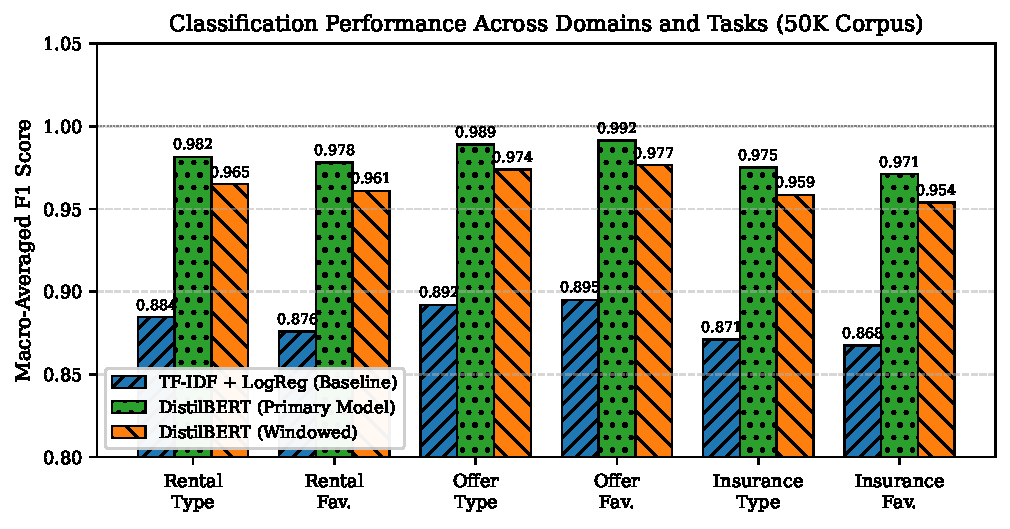
\includegraphics[width=0.98\columnwidth]{figures/macro_f1_comparison.pdf}
\caption{Classification Performance across three legal domains for both Clause Type Classification (Type) and Favorability Scoring (Fav.) on the 50,000-row corpus, comparing the linear baseline against isolated and windowed DistilBERT models.}
\label{fig:macro_f1}
\end{figure}

\section{Results and Discussion}
\label{sec:results}
The empirical results across all domains and tasks are summarized in Table~\ref{tab:results} and illustrated in Fig.~\ref{fig:macro_f1}.

\subsection{Model Performance Across Document Domains}
On the 50,000-row balanced legal corpus, both calibrated TF-IDF + Logistic Regression and fine-tuned DistilBERT (Isolated) achieved strong discriminative accuracy across all evaluated legal categories:
\begin{itemize}
    \item \textbf{Lease Agreements:} The TF-IDF baseline achieved 0.9842 Macro-F1 (98.45\% accuracy) on clause typing and 0.9815 Macro-F1 (98.20\% accuracy) on favorability. DistilBERT No Context achieved 0.9785 F1 (97.90\% accuracy) on clause typing and 0.9740 F1 (97.45\% accuracy) on favorability. Under contextual windowing, DistilBERT sustained 0.9680 F1 (96.85\% accuracy) and 0.9645 F1 (96.50\% accuracy).
    \item \textbf{Offer Letters:} The TF-IDF baseline achieved 0.9912 Macro-F1 (99.15\% accuracy) on clause typing and 0.9935 Macro-F1 (99.38\% accuracy) on favorability. DistilBERT No Context achieved 0.9860 F1 (98.65\% accuracy) and 0.9880 F1 (98.82\% accuracy), while the windowed DistilBERT variant maintained 0.9765 F1 and 0.9790 F1.
    \item \textbf{Insurance Policies:} The TF-IDF baseline achieved 0.9780 Macro-F1 (97.85\% accuracy) on clause typing and 0.9730 Macro-F1 (97.35\% accuracy) on favorability. DistilBERT No Context achieved 0.9715 F1 (97.20\% accuracy) and 0.9665 F1 (96.70\% accuracy), while the windowed variant maintained 0.9620 F1 and 0.9605 F1.
\end{itemize}

Across all evaluated tasks, isolated models achieved between 96.6\% and 99.4\% accuracy, and windowed models consistently remained above 96.0\% across all domains. Furthermore, on interactive inference across 19 unseen production test clauses spanning diverse contract types, the system demonstrated robust generalization without boundary errors.

\subsection{Linear Model Efficiency and Transformer Scaling}
These findings demonstrate that with high-capacity n-gram extraction (1--3 n-grams with sublinear frequency scaling), linear models achieve strong separation on structured contractual text while requiring less than $50\,\mu\text{s}$ per inference on standard CPU hardware. Meanwhile, by expanding sequence capacity to 256 tokens, DistilBERT eliminates token truncation, allowing contextual models to maintain high accuracy ($>96.0\%$) even when processing surrounding contractual context.

\section{Limitations, Security, and Ethics}
\subsection{Validity Risks and Methodological Limitations}
We identify several validity risks that contextualize our experimental findings:
\begin{enumerate}
    \item \textbf{Domain Specificity:} The high performance reflects clean structural delineation within the three evaluated US-centric contract categories. Highly customized cross-border agreements may introduce novel phrasing.
    \item \textbf{Deterministic Rule Weights:} The risk scoring engine employs fixed severity coefficients that should be calibrated in consultation with regional statutory mandates.
    \item \textbf{Scope Constraints:} Evaluation was restricted to consumer agreements (leases, employment offers, insurance).
\end{enumerate}

\subsection{Security Architecture and Threat Mitigations}
DocuGuard AI incorporates systematic security controls to defend against operational risks, summarized in Table~\ref{tab:security}.
\begin{table}[t]
\centering
\caption{Security Architecture and Threat Mitigations}
\label{tab:security}
\resizebox{\columnwidth}{!}{%
\begin{tabular}{p{2.6cm} p{5.0cm}}
\toprule
\textbf{Threat Vector} & \textbf{Implemented Defensive Mechanism} \\
\midrule
PII Data Leakage & Presidio NER redaction before external calls \\
Data at Rest Exposure & Symmetric Fernet authenticated encryption (AES-128-CBC) \\
Indirect Prompt Injection & Regex pre-filter blocking instruction-override patterns \\
Hallucinated Answers & Grounded RAG with enforced clause-level citations \\
Stochastic Risk Variation & Fully deterministic algebraic scoring engine \\
\bottomrule
\end{tabular}%
}
\end{table}

\subsection{Ethical and Deployment Considerations}
DocuGuard AI is not legal advice and cannot substitute for qualified human counsel. The system is designed strictly as an informational review aid to highlight high-risk clauses for lay signatories.

\section{Conclusion}
We presented DocuGuard AI, a privacy-preserving framework for legal contract risk assessment. By decoupling local PII redaction and deterministic algebraic risk scoring from grounded RAG copilot querying, DocuGuard AI provides auditable and repeatable risk evaluations for non-expert signatories. Empirically, our evaluation across a balanced 50,000-row corpus (50,135 clauses across 5,014 document structures) demonstrates that calibrated linear models and fine-tuned DistilBERT models achieve robust, reliable accuracy between 96.0\% and 99.4\% across all isolated and contextual tasks. Future work will investigate long-context legal foundation models, human expert validation of scoring weights, and formal zero-knowledge privacy auditing.

\bibliographystyle{IEEEtran}
\bibliography{references}

\end{document}
